%===========================================================================
%	Einleitung
%===========================================================================
\section{Marktüberblick}

Marktanteile / Nutzung von Mobilgeräten

Für das Jahr 2020 wird erwartet, dass 45\% der Weltbevölkerung ein Smartphone nutzt.
% https://www.statista.com/statistics/330695/number-of-smartphone-users-worldwide/
\cite{StatistaSmartphonesWorldwide}
%https://www.statista.com/statistics/262875/development-of-the-world-population/
\cite{StatistaWorldPopulation}
% 3,5 / 7,79 Milliarden = 45%
Sowohl Unternehmen, die ihre Produkte überwiegend offline vertreiben, als auch die führenden IT-Unternehmen wissen um diesen Trend, denn App-Nutzer sind (potenzielle) Kunden. Auch die Medienbranche verdient mit App-Nutzern Geld, da mit jedem Nutzer ihrer Website oder App die Werbeeinnahmen steigen. 
Newsportale wie Focus Online, BILD, Welt.de oder Spiegel Online gehören 2019 zu den verbreitetsten mobilen Webseiten \cite{StatistaMobileWebsiteNetReach2019}. Diese  Webseiten sind bereits für Mobilegeräte optimiert. Für Entwickler liegt es nahe, die Webseite in einer Mobilanwendung einzubetten, anstatt alle Features in einer nativen Anwendung neu zu entwickeln. Der Nutzer kann diese Anwendungen über einen App Marktplatz beziehen. Mit Bannern und Links versuchen Unternehmen auf ihre Mobilanwendungen aufmerksam zu machen.
Mit dem Konzept der \ac{pwa} könnte dieser Schritt bald obsolet werden, wenn Nutzer nicht mehr eine plattformabhängige App, sondern vielmehr die Webseite selbst als ``Anwendung'' installieren. Bezieht man die vergleichsweise hohen Entwicklungskosten mobiler Anwendungen in diese Rechnung mit ein, besteht eine große Chance, dass die Erweiterung der bestehenden Webseite zur PWA schneller, wartungärmer und insgesamt günstiger ist.

Die Progressive Web App verspricht nicht nur einen einfachen Container um eine Website, sondern auch Offline-Funktionalität, vergleichsweise einfache Entwicklung mit JavaScript und Unabhängigkeit der Plattform. Damit löst sie viele bekannte Probleme einfacher Container Apps um eine Webseite. Nicht selten wird dort die Geduld der Nutzer herausgefordert, da alle Inhalte (Scripte, Stylesheets, Schriftarten, HTML etc.) ständig über eine möglicherweise langsame Datenverbindung heruntergeladen werden müssen.

Der Hohe Marktanteil (60\% in 2019) des mobilen Browsers Google Chrome (welcher die Installation von PWAs voll unterstützt \cite[S. 8]{BeginningPWA}) und Apples Safari für iOS (20\% in 2019), welcher die Unterstützung der PWA stetig erweitert, inspirieren diese Arbeit, die Möglichkeiten der PWA im Vergleich zur nativen App ausführlich zu vergleichen.
\cite{StatistaMobileBrowserMarketShare}

% Mobile shopping app user acquisition costs
%https://www.statista.com/statistics/911981/mobile-shopping-apps-user-acquisition-costs-by-type-gender/

% median cost of app dev in regions by $ per hour$
%https://www.statista.com/statistics/628636/worldwide-mobile-app-development-costs-by-region-by-platform/

% median cost of app dev per hour
%https://www.statista.com/statistics/647807/north-america-mobile-app-development-costs/

% market share mobile browsers
%https://www.statista.com/statistics/263517/market-share-held-by-mobile-internet-browsers-worldwide/

% Leading mobile websites ranked by net reach in Germany
%https://www.statista.com/statistics/425372/mobile-websites-by-net-reach-germany/


%\begin{figure}[h]
%        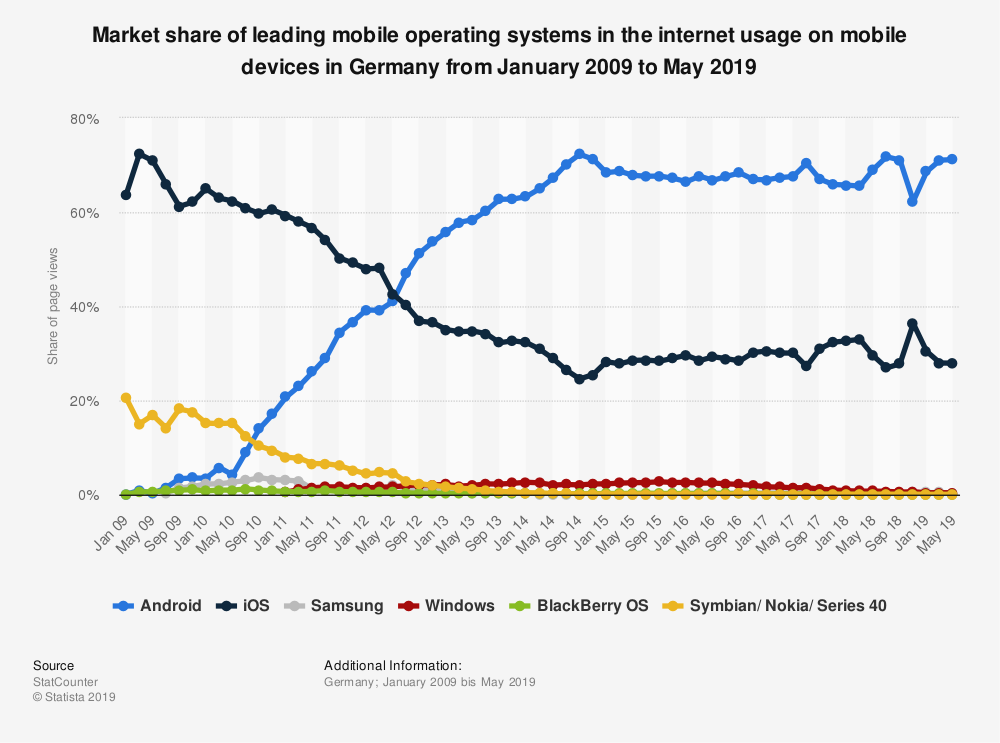
\includegraphics[width=\linewidth]{img/statistic_id461981_market-share-of-operating-systems-in-mobile-internet-usage-in-germany-2009-2019.png}
%        \centering
%        \caption{Market share \cite{StatistaMarketShareSmartphone}}
%        \label{fig:marketshare}
%\end{figure}

%===========================================================================
%	Motivation
%===========================================================================
\section{Motivation dieser Arbeit}
Forschungsfrage: kann \ac{pwa} native App langfristig ablösen

Mobilegeräte Leistungsstärker
Möglichkeiten plattformübergreifend zu entwickeln

Nutzer Conversion kann langfristig gesteigert werden --> Profit!\\
https://developers.google.com/web/progressive-web-apps
\cite{GooglePWAOverview}



%===========================================================================
%	Kapitelübersicht
%===========================================================================
\section{Kapitelübersicht}
In diesem Kapitel (\ref{chap:einleitung}) wurden die aktuellen Marktenwicklungen kurz mit Zahlen benannt und die Motivation dieser Arbeit dargelegt. Das folgende Kapitel 
(\ref{chap:grundlagen} \nameref{chap:grundlagen}) legt vorwiegend technischen Grundlagen für die spätere Implementierung einer Anwendung als PWA und nativer App. Dabei wird auf die verwendeten Technologien und Frameworks eingegangen und speziell die PWA auf technischer Ebene erklärt. 

Kapitel \ref{chap:architektur} (\nameref{chap:architektur}) erläutert die Architektur der entwickelten Anwendung: eine Todoliste. In diesem Kapitel werden detaillierte Spezifikationen beschrieben, die den Entwicklungsprozess erst vergleichbar machen. Außerdem wird auf architekturbezogene Entscheidungen der Plattformen eingegangen, beispielsweise die Gründe für die Wahl der Frameworks der PWA.

Um den Entwicklungsprozess vergleichen zu können, wird in Kapitel \ref{chap:framework} (\nameref{chap:framework}) der Vergleichsprozess beschrieben und Kriterien mit ihrer Gewichtung aufgestellt und erläutert. Anschließend werden im zweigeteilten Kapitel \ref{chap:implementierung} (\nameref{chap:implementierung}) die Implementierungsprozesse der PWA und der nativen App detailliert dokumentiert.

Nach dem Sammeln von Erfahrungen bei den Implementierungen werden in Kapitel \ref{chap:evaluation} (\nameref{chap:evaluation}) beide Technologien mithilfe der in Kapitel \ref{fig:marketshare} erstellten Kriterien verglichen und evaluiert.

Abschließend gibt Kapitel \ref{chap:reflexion} (\nameref{chap:reflexion}) ein Urteil über den Erfolg dieser Arbeit und gibt einen Ausblick auf die Zukunft der PWA.
